% Options for packages loaded elsewhere
\PassOptionsToPackage{unicode}{hyperref}
\PassOptionsToPackage{hyphens}{url}
%
\documentclass[
  a4paper,
]{scrbook}

\usepackage{amsmath,amssymb}
\usepackage{iftex}
\ifPDFTeX
  \usepackage[T1]{fontenc}
  \usepackage[utf8]{inputenc}
  \usepackage{textcomp} % provide euro and other symbols
\else % if luatex or xetex
  \usepackage{unicode-math}
  \defaultfontfeatures{Scale=MatchLowercase}
  \defaultfontfeatures[\rmfamily]{Ligatures=TeX,Scale=1}
\fi
\usepackage{lmodern}
\ifPDFTeX\else  
    % xetex/luatex font selection
  \setmainfont[]{Latin Modern Roman}
  \setsansfont[]{Latin Modern Roman}
\fi
% Use upquote if available, for straight quotes in verbatim environments
\IfFileExists{upquote.sty}{\usepackage{upquote}}{}
\IfFileExists{microtype.sty}{% use microtype if available
  \usepackage[]{microtype}
  \UseMicrotypeSet[protrusion]{basicmath} % disable protrusion for tt fonts
}{}
\makeatletter
\@ifundefined{KOMAClassName}{% if non-KOMA class
  \IfFileExists{parskip.sty}{%
    \usepackage{parskip}
  }{% else
    \setlength{\parindent}{0pt}
    \setlength{\parskip}{6pt plus 2pt minus 1pt}}
}{% if KOMA class
  \KOMAoptions{parskip=half}}
\makeatother
\usepackage{xcolor}
\setlength{\emergencystretch}{3em} % prevent overfull lines
\setcounter{secnumdepth}{5}
% Make \paragraph and \subparagraph free-standing
\ifx\paragraph\undefined\else
  \let\oldparagraph\paragraph
  \renewcommand{\paragraph}[1]{\oldparagraph{#1}\mbox{}}
\fi
\ifx\subparagraph\undefined\else
  \let\oldsubparagraph\subparagraph
  \renewcommand{\subparagraph}[1]{\oldsubparagraph{#1}\mbox{}}
\fi


\providecommand{\tightlist}{%
  \setlength{\itemsep}{0pt}\setlength{\parskip}{0pt}}\usepackage{longtable,booktabs,array}
\usepackage{calc} % for calculating minipage widths
% Correct order of tables after \paragraph or \subparagraph
\usepackage{etoolbox}
\makeatletter
\patchcmd\longtable{\par}{\if@noskipsec\mbox{}\fi\par}{}{}
\makeatother
% Allow footnotes in longtable head/foot
\IfFileExists{footnotehyper.sty}{\usepackage{footnotehyper}}{\usepackage{footnote}}
\makesavenoteenv{longtable}
\usepackage{graphicx}
\makeatletter
\def\maxwidth{\ifdim\Gin@nat@width>\linewidth\linewidth\else\Gin@nat@width\fi}
\def\maxheight{\ifdim\Gin@nat@height>\textheight\textheight\else\Gin@nat@height\fi}
\makeatother
% Scale images if necessary, so that they will not overflow the page
% margins by default, and it is still possible to overwrite the defaults
% using explicit options in \includegraphics[width, height, ...]{}
\setkeys{Gin}{width=\maxwidth,height=\maxheight,keepaspectratio}
% Set default figure placement to htbp
\makeatletter
\def\fps@figure{htbp}
\makeatother

\usepackage{booktabs}
\usepackage{longtable}
\usepackage{array}
\usepackage{multirow}
\usepackage{wrapfig}
\usepackage{float}
\usepackage{colortbl}
\usepackage{pdflscape}
\usepackage{tabu}
\usepackage{threeparttable}
\usepackage{threeparttablex}
\usepackage[normalem]{ulem}
\usepackage{makecell}
\usepackage{xcolor}
\usepackage{titling}
\setlength{\droptitle}{-2cm}
\preauthor{
  \begin{center}
  \Large
  \vspace{10mm}
  by

  \vspace{20mm}
}
\postauthor{
  \end{center}
  \vfill
}

\predate{
  \begin{center}
  A thesis 
  submitted in fulfilment of the \\
  requirements of the degree of \\
  Doctor of Philosophy in Physics\\               % Degree
  School of Physical and Chemical Sciences\\          % Department
  Te Herenga Waka - Victoria University of Wellington\\                       % University 
  \vspace{5mm}
}
\postdate{
  \\
  
\includegraphics[width=3in,height=1.5in]{figures/VUW-logo.png}\\
  \end{center}
  }
\makeatletter
\makeatother
\makeatletter
\@ifpackageloaded{bookmark}{}{\usepackage{bookmark}}
\makeatother
\makeatletter
\@ifpackageloaded{caption}{}{\usepackage{caption}}
\AtBeginDocument{%
\ifdefined\contentsname
  \renewcommand*\contentsname{Table of contents}
\else
  \newcommand\contentsname{Table of contents}
\fi
\ifdefined\listfigurename
  \renewcommand*\listfigurename{List of Figures}
\else
  \newcommand\listfigurename{List of Figures}
\fi
\ifdefined\listtablename
  \renewcommand*\listtablename{List of Tables}
\else
  \newcommand\listtablename{List of Tables}
\fi
\ifdefined\figurename
  \renewcommand*\figurename{Figure}
\else
  \newcommand\figurename{Figure}
\fi
\ifdefined\tablename
  \renewcommand*\tablename{Table}
\else
  \newcommand\tablename{Table}
\fi
}
\@ifpackageloaded{float}{}{\usepackage{float}}
\floatstyle{ruled}
\@ifundefined{c@chapter}{\newfloat{codelisting}{h}{lop}}{\newfloat{codelisting}{h}{lop}[chapter]}
\floatname{codelisting}{Listing}
\newcommand*\listoflistings{\listof{codelisting}{List of Listings}}
\makeatother
\makeatletter
\@ifpackageloaded{caption}{}{\usepackage{caption}}
\@ifpackageloaded{subcaption}{}{\usepackage{subcaption}}
\makeatother
\makeatletter
\@ifpackageloaded{tcolorbox}{}{\usepackage[skins,breakable]{tcolorbox}}
\makeatother
\makeatletter
\@ifundefined{shadecolor}{\definecolor{shadecolor}{rgb}{.97, .97, .97}}
\makeatother
\makeatletter
\makeatother
\makeatletter
\makeatother
\ifLuaTeX
  \usepackage{selnolig}  % disable illegal ligatures
\fi
\usepackage[citestyle = ieee,urldate = iso8601]{biblatex}
\addbibresource{references.bib}
\IfFileExists{bookmark.sty}{\usepackage{bookmark}}{\usepackage{hyperref}}
\IfFileExists{xurl.sty}{\usepackage{xurl}}{} % add URL line breaks if available
\urlstyle{same} % disable monospaced font for URLs
\hypersetup{
  pdftitle={Developing an Insect Odorant Receptor Bioelectronic Nose for Vapour-Phase Detection},
  pdfauthor={Eddyn Oswald Perkins Treacher},
  hidelinks,
  pdfcreator={LaTeX via pandoc}}

\title{Developing an Insect Odorant Receptor Bioelectronic Nose for
Vapour-Phase Detection}
\author{Eddyn Oswald Perkins Treacher}
\date{May 2024}

\begin{document}
\frontmatter

\maketitle

\clearpage
\newpage
\thispagestyle{empty} % Hide header and footer on this page
\mbox{~}
\clearpage
\newpage

%----------------------------------------------
%   Abstract
%----------------------------------------------

\begin{flushleft}
% Manually add a section to the table of contents
\pagenumbering{roman}
\addcontentsline{toc}{chapter}{Abstract}
\huge\textbf{Abstract}
\end{flushleft}

\vspace*{\baselineskip}

This is a thesis skeleton written with quarto.
Make a copy of this thesis repo and start to write!

Make a new paragraph by leaving a blank line.

\clearpage
\newpage
\thispagestyle{empty} % Hide header and footer on this page
\mbox{~}
\clearpage
\newpage


%----------------------------------------------
%   Acknowledgement
%----------------------------------------------

\begin{flushleft}
% Manually add a section to the table of contents
\addcontentsline{toc}{chapter}{Acknowledgements}
\huge\textbf{Acknowledgements}
\end{flushleft}

\vspace*{\baselineskip}

B3 partnership!

At the university

Rifat, Alex - vapour sensor design and construction
Peter Coard - electronics work
Erica Cassie - FET sensing setup
Rob Keyzers and Jennie Ramirez-Garcia - NMR spectra
Patricia Hunt - Computational chemistry
Erica Happe - steaming method
Danica- AFM imaging
Sushila Pillai - Fluorescence microscope training
Jenna and Ali - Device functionalisation

Interns
Lotte Boer
Liam Anderson
Hayden Young

Nick Grinter - vapour sensor setup
Grant Franklin - vapour sensor setup
Alan Rennie and Alex Puglisi - vapour sensor setup

Family and friends

Oldest friends - Bennett, Jaquille
High school friends
Undergrad friends
Friends on Discord
Je - gym
Aikido group (Ian, Lee, Jak, Tim)
Extended whanau
Mum and Dad
Nina!

\clearpage
\newpage
\thispagestyle{empty} % Hide header and footer on this page
\mbox{~}
\clearpage
\newpage

\ifdefined\Shaded\renewenvironment{Shaded}{\begin{tcolorbox}[frame hidden, enhanced, breakable, sharp corners, borderline west={3pt}{0pt}{shadecolor}, interior hidden, boxrule=0pt]}{\end{tcolorbox}}\fi

\renewcommand*\contentsname{Table of Contents}
{
\setcounter{tocdepth}{2}
\addcontentsline{toc}{chapter}{Table of Contents}
\tableofcontents
}
\listoffigures
\addcontentsline{toc}{chapter}{List of Figures}
\listoftables
\addcontentsline{toc}{chapter}{List of Tables}

\clearpage
\newpage
\thispagestyle{empty} % Hide header and footer on this page
\mbox{~}
\clearpage
\newpage

%----------------------------------------------
%   List of Abbreviations
%----------------------------------------------

\thispagestyle{plain} % Hide header and footer on this page

\begin{flushleft}
% Manually add a section to the table of contents
\addcontentsline{toc}{chapter}{List of Abbreviations}
\huge\textbf{List of Abbreviations}
\end{flushleft}

\vspace*{\baselineskip}

\begin{table}[h]
  \begin{tabular}{@{}p{0.25\textwidth} p{0.75\textwidth}@{}}  % Adjust the width as needed
    Ab  & Antibody  \\
    AB  & Amyl Butyrate  \\
    AFM  & Atomic Force Microscope  \\
    Avi-tag  & Avidin-tag  \\
    BMIM  & 1-Butyl-3-methylimidazolium bis(trifluoromethylsulfonyl)imide  \\
    CNT  & Carbon Nanotube  \\
    CVD  & Chemical Vapour Deposition  \\
    DAN  & 1,5-diaminonaphthalene  \\
    DMT-MM   & 4-(4,6-dimethoxy-1,3,5-triazin-2-yl)-4 methylmorpholinium chloride \\
    DMMP  & Dimethyl Methylphosphonate  \\
    DNA  & Deoxyribonucleic Acid  \\
    EB  & Ethyl Butyrate  \\
    EDL  & Electric Double Layer  \\
    FET  & Field-Effect Transistor  \\
    GA  & Glutaraldehyde  \\
    GFET  & Graphene Field-Effect Transistor  \\
    GPCR  & G-protein Coupled Receptor  \\
    HEK  & Human Embryonic Kidney  \\
    His-tag  & Histidine-tag  \\
    hOR  & Human Odorant Receptor  \\
    iOR  & Insect Odorant Receptor  \\
    LOD  & Limit of Detection  \\
    m-CNT  & Metallic Carbon Nanotube   \\
    mOR  & Mouse Odorant Receptor  \\
    MOSFET  & Metal-Oxide-Semiconductor Field-Effect Transistor  \\
    MSP  & Membrane Scaffold Protein  \\
    MWCNT  & Multi-Walled Carbon Nanotube   \\
    NSB  & Non-Specific Binding   \\
    NTA  & Nitrilotriacetic Acid   \\
    OBP  & Odorant Binding Protein  \\
    OR  & Odorant Receptor  \\
    ORCO  & Odorant Receptor Co-Receptor  \\
    PBASE  & 1-Pyrenebutanoic Acid N-hydroxysuccinimide Ester  \\ 
  \end{tabular}
\end{table}

\newpage
\pagestyle{plain} % Hide header and footer on this page
\begin{table}[h]
  \begin{tabular}{@{}p{0.25\textwidth} p{0.75\textwidth}@{}}  % Adjust the width as needed
    PBS  & Phosphate-Buffered Saline  \\
    PDL & Poly-\textit{D}-lysine  \\
    PDMS  & Polydimethylsiloxane   \\ 
    PEG  & Polyethylene Glycol  \\ 
    PLL & Poly-\textit{L}-lysine  \\
    ppb & parts per billion  \\
    ppm & parts per million  \\
    ppt & parts per trillion  \\
    RNA  & Ribonucleic Acid   \\ 
    s-CNT  & Semiconducting Carbon Nanotube   \\
    SEM  & Scanning Electron Microscope   \\
    SWCNT  & Single-Walled Carbon Nanotube   \\
    TFTFET  & Thin-Film Field-Effect Transistor  \\
    TX  & Transfer Characteristics  \\
    VUAA1  & N-(4-Ethylphenyl)-2-{[4-ethyl-5-(pyridin-3-yl)-4H-1,2,4-triazol-3-yl]sulfanyl}acetamide  \\ 
  \end{tabular}
\end{table}

\clearpage
\newpage
\thispagestyle{empty} % Hide header and footer on this page
\mbox{~}
\clearpage
\newpage

\mainmatter
\bookmarksetup{startatroot}

\hypertarget{introduction}{%
\chapter{Introduction}\label{introduction}}

My aim is to develop a `bioelectronic nose', a biosensor device which
couples sensitive biological recognition elements with an electronic
transducer for the detection of vapour phase compounds
\autocite{Lee2010,Dung2018,Moon2020}. The transducer converts the
interaction or interactions between the recognition element and analyte
or analytes of interest into a measureable electronic signal. The
sensitive biological component used here are \emph{Drosophila
melanogaster} insect odorant receptors (iORs), while the electronic
transducer element is a carbon nanotube- or graphene-based field effect
transistor (CNTFET or GFET). Carbon-based 2D nanomaterials are promising
for use in novel biosensors as they are highly sensitive, biocompatible
and cheap to fabricate \autocite{Shkodra2021}. I created a purpose-built
vapour delivery system apparatus in order to test these devices.
Initially, however, iOR-functionalised CNTFETs and GFETs (iOR-FETs) were
first tested in the liquid phase to corroborate previous findings within
my research group \autocite{Murugathas2019a,Murugathas2020}.

There has been a significant amount of work done towards creating
bioelectronic noses over the last twenty years. This is largely due to
their promisingly high level of sensitivity and specificity in real-time
in the gas phase, with the ability to signal the presence of volatile
organic compound (VOC) traces at lower concentrations than traditional
chemical sensors or the human nose in a timescale of seconds
\autocite{Lee2010,Moon2020,Terutsuki2020}. The implications of
successful development of a portable and robust bioelectronic nose are
significant and varied. Applications could be found in high-importance
fields such as biosecurity, medicine, environmental protection and food
or water safety \autocite{Dung2018,Arakawa2019,Yang2017,Son2017}. It has
been demonstrated that it is possible to detect invasive brown
marmorated stinkbugs based on their volatile trace \autocite{Moser2020}.
A bioelectronic nose could potentially accomplish this task far more
cheaply and efficiently than trained sniffer dogs.

As well as a variety of practical applications, development of a
bioelectronic nose may give us a greater understanding of the mechanisms
underlying insect olfaction, as well as novel understandings of the
transducer devices used to register the electronic response to VOCs
\autocite{Lee2010}. The transduction mechanism of nanomaterial-based iOR
sensors is still unknown, and I hope to shed further light on the
biological and electronic processes underpinning this mechanism
\autocite{Murugathas2020,Khadka2019}.

\bookmarksetup{startatroot}

\hypertarget{sec-iOR-sensors}{%
\chapter{Biosensing with Insect Odorant
Receptors}\label{sec-iOR-sensors}}

\hypertarget{sec-biosensing-transducers}{%
\section{Introduction}\label{sec-biosensing-transducers}}

In \textbf{?@sec-thin-film-transistors}, it was established that as
carbon nanotubes and graphene are highly sensitive and are easily
modified with biomaterials, they make an ideal platform for biosensing
\autocite{Kauffman2008,Ohno2010}. In the early 2000s, it was established
that sensitive and selective biosensors could be created by modifying a
carbon nanotube field-effect transistor channel with protein receptors
\autocite{Chen2003,Kauffman2008}. In the following two decades, a wide
range of other biological receptors have been attached to carbon
nanotube FETs and graphene FETs for the creation of biosensors,
including enzymes \autocite{Lee2009,Zhang2015a,Dudina2019}, antibodies
\autocite{Kim2008,Jin2015,Tsang2019} and aptameric DNA
\autocite{Maehashi2007,Gao2016,Nguyen2021}. These miniaturised `lab on a
chip' devices are of particular interest due to their reliability, low
cost, rapid use time, simple operation and small size compared with more
traditional biological analysis methods
\autocite{Kauffman2008,Khan2020}. It is hoped that such sensors could be
deployed outside the laboratory in a range of front-line settings
requiring rapid and reliable detection
\autocite{Dung2018,Yang2018,Kim2022a}.

Rapid developments in this biosensor technology and parallel
developments in the understanding of animal olfaction led to these
transistors being used in bioelectronic nose applications from the late
2000s onwards \autocite{Yoon2009,Jin2012,Lee2012b,Park2012}.
`Bioelectronic nose' is a general term dating back to 1961, which refers
to the use of an biologically-modified electronic array to detect
specific odor traces in a highly selective and sensitive manner. As the
name suggests, the signals from this system mimic the electrochemical
signals received by olfactory neurons in an animal nose
\autocite{Glatz2011,Dung2018}. A biomimetic approach to bioelectronic
nose development couples the CNT FET or GFET signal-amplifying
transducer element with sensitive components of the animal olfactory
system. These components include olfactory cells \autocite{Wang2007},
odorant binding proteins (OBPs) \autocite{Larisika2015,Kotlowski2018}
and odorant receptor proteins (olfactory receptors, ORs)
\autocite{Yang2018,Murugathas2020}. An animal nose can discern specific
volatile odors in the air at low parts-per-trillion concentrations,
performance which is far superior to even the best available gas sensor
technology. The aim for novel olfactory-based electronic biosensors is
to match or surpass this level of selective accuracy
\autocite{Glatz2011,Kwon2015,Dung2018,Bohbot2020,Kim2022a}.

\hypertarget{sec-odorant-receptors-biosensors}{%
\section{Odorant Receptors in Field-Effect Transistor
Biosensors}\label{sec-odorant-receptors-biosensors}}

\hypertarget{sec-odorant-receptors}{%
\subsection{Odorant Receptors}\label{sec-odorant-receptors}}

Odorant receptors (ORs) are an essential part of the olfactory systems
of most animals, including humans. ORs let us distinguish between
thousands of odors \autocite{Buck1991,Dung2018,Yang2018,Kim2022a}.
Vertebrate odorant receptors are part of a group of seven-transmembrane
proteins known as G-protein coupled receptors (GPCRs)
\autocite{Buck1991,Glatz2011,Dung2018,Wicher2021}. Compounds entering a
vertebrate nose selectively bind to specific odorant receptors, which
undergo a change in conformation \autocite{Dung2018,Kim2022a}. The
binding process leads to activation and dissociation of the G-protein
within the neuronal cell. Intracellular signalling events triggered by
G-protein dissociation are converted to an action potential which is
then transmitted to the brain \autocite{Buck1991,Glatz2011,Zhang2021}.
The combination of activated receptors is then interpreted as a specific
odor \autocite{Sato2014,Kwon2015,Hurot2020,Kim2022a}. Odorant receptors
may be activated by a few or many target (or `agonist') compounds. The
target compounds are determined by subtle differences in OR amino acid
composition \autocite{Carraher2015,Yang2018,Goodwin2021}. An
`antagonist' compound may inhibit the response of a receptor to other
compounds \autocite{Lee2012,Carraher2015}. Compounds which trigger a
strong signal from a specific odorant receptor are often referred to as
`positive ligands' for that receptor, while those that cause no response
are `negative ligands'
\autocite{Murugathas2019a,Murugathas2020,Yoo2022}.

\hypertarget{sec-artificial-membranes}{%
\subsection{Artificial Membranes}\label{sec-artificial-membranes}}

Odorant receptors are transmembrane proteins, which are insoluble and
tend to aggregate and oligomerise in solution \autocite{Nath2007}. They
therefore require stabilisation from either a specific detergent
environment or a membrane layer to preserve their structure and function
when solubilised \autocite{Fruh2011,Dung2018}. Odorant receptors can be
expressed and isolated using heterologous cell systems, where a host
cell replicates a protein from transfected RNA or DNA material
\autocite{Glatz2011,Dung2018}. The most commonly used expression cells
are human embryonic kidney (HEK) cells \autocite{Lim2014,Ahn2020},
\emph{E. Coli} bacteria \autocite{Yang2017,Yang2018} and \emph{S.
cerevisiae} (baker's yeast) \autocite{Bohbot2020}. The cell membrane can
then be used directly in a sensor \autocite{Dung2018}. Alternatively,
odorant receptors can be embedded in an artificial lipid membrane format
that mimics the native cell membrane \autocite{Nath2007}. These
membranes can be produced in large numbers and remain in storage for
much longer than live cells \autocite{Goldsmith2011,Lim2015}. Lipid
membranes are constructed from phospholipid molecules, which comprise of
a small, hydrophilic, polar `head' and long, hydrophobic, non-polar
`tail' \autocite{Bose2021,Ramadon2022}. These artificial membranes
include detergent micelles, nanovesicles (including liposomes), and
nanodiscs \autocite{Yang2018,Moon2020}. The small size of these
artificial membranes makes them appropriate for use with
nanomaterial-based transducers \autocite{Lim2015,Dung2018}.

\begin{figure}

{\centering 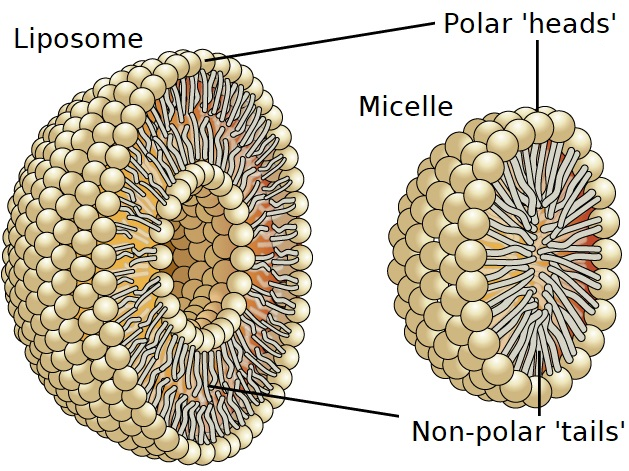
\includegraphics[width=0.53\textwidth,height=\textheight]{figures/ch3/OSC_Microbio_07_03_micelle_edit.png}

}

\caption{\label{fig-micelle}Liposomes and micelles are made up of a
lipid membrane, which acts as a substitute for the cell membrane
\emph{in vitro}. The polar, hydrophilic `heads' and non-polar,
hydrophobic `tails' of the component phospholipids are indicated.
Adapted from \autocite{Micelle}.}

\end{figure}

A nanovesicle is a nanoscopic spherical bilayer fluid sac. There are
various types of artificial nanovesicles, including liposomes,
ethosomes, transfersomes, niosomes and phytosomes. The type of
nanovesicle depends on its chemical makeup \autocite{Ramadon2022}. For
example, a liposome is made up of phospholipid and cholesterol, and can
consist of one or more concentric amphiphilic bilayers. The liposome can
contain hydrophobic compounds within the bilayer due to hydrophobic
interactions, while hydrophilic compounds are held within the vesicle
core or interior \autocite{Nath2007,Ramadon2022}. A nanovesicle can be
used solely as a format to protect membrane proteins
\autocite{Murugathas2020}, or with the addition of integrated ion
channels, can mimic the operation of a cell \emph{in vivo}, with
intracellular signalling pathways triggered by the membrane proteins
\autocite{Lim2015}. Nanomicelles (or simply micelles) are also
nanoscopic and spherical, but unlike nanovesicles have no inner fluid
sac \autocite{Nath2007,Bose2021}. Micelles self-assemble when
phospholipid is mixed with detergent. The surface of the micelle is made
up of the hydrophilic detergent and phospholipid heads, while the
internal core is made up of the hydrophobic phospholipid tail
\autocite{Nath2007}. Hydrophobic compounds can be contained within the
core of the micelle \autocite{Bose2021}. Figure~\ref{fig-micelle}
illustrates the difference between the liposome and micelle structures.

\begin{figure}

{\centering 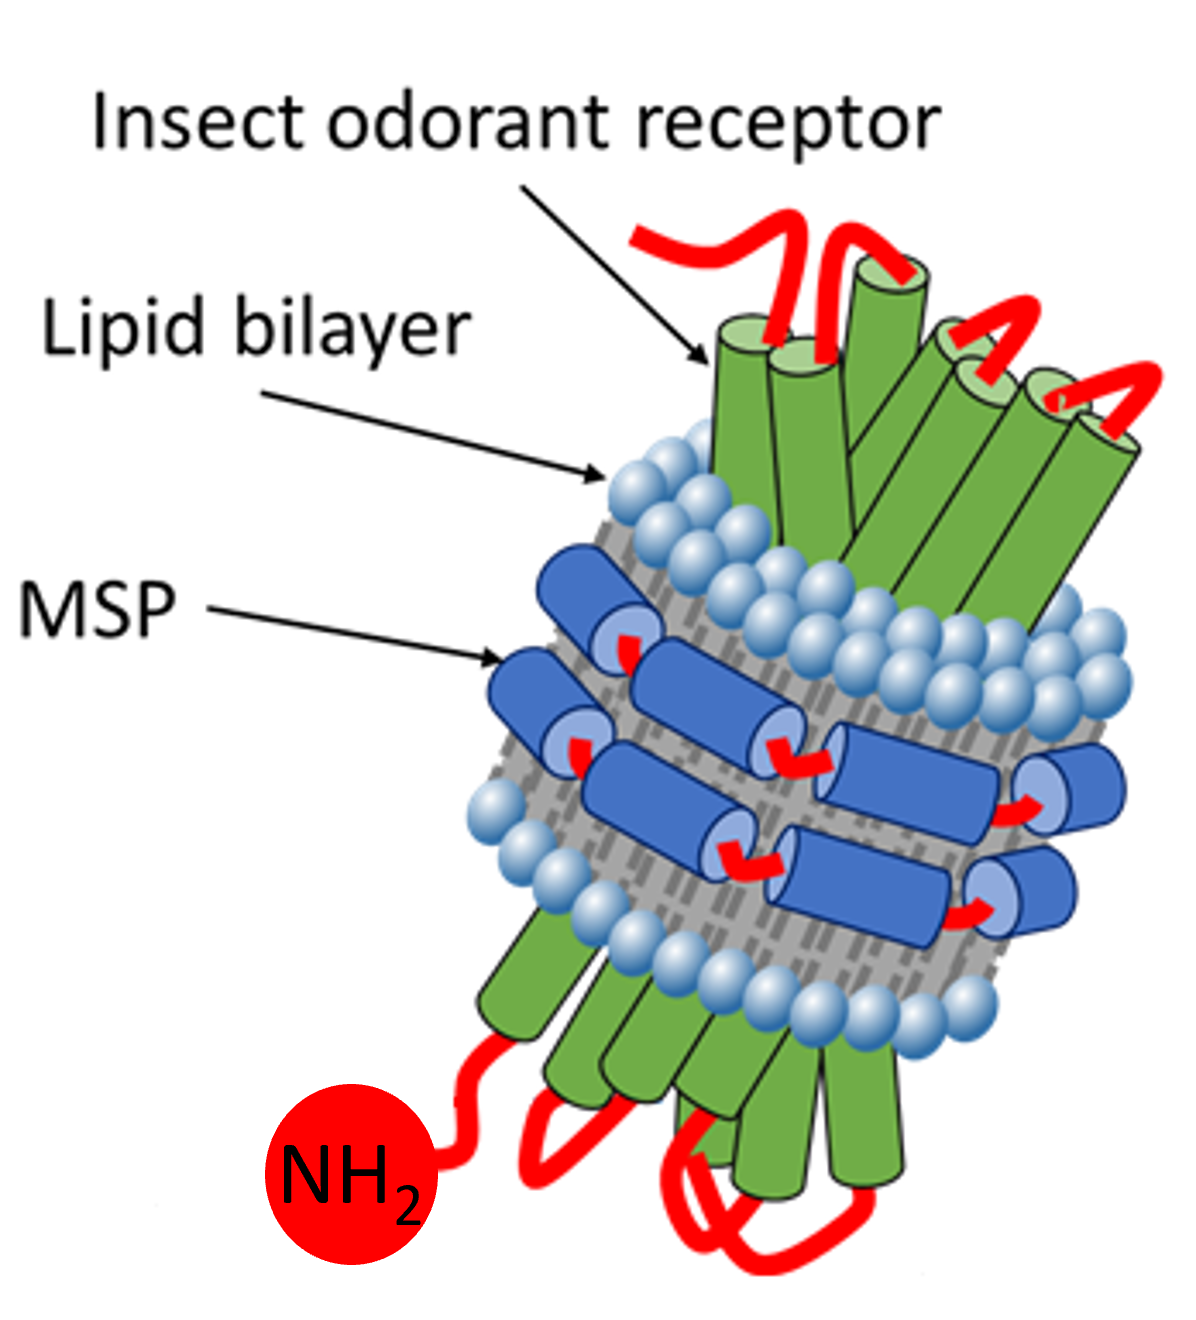
\includegraphics[width=0.4\textwidth,height=\textheight]{figures/ch3/iOR_nanodisc.png}

}

\caption{\label{fig-msp-iOR-nanodisc}A nanodisc containing an insect
odorant receptor transmembrane protein. The amine group shown is the
odorant receptor N-terminus. Reproduced with permission from
\autocite{Murugathas2019a}.}

\end{figure}

Nanodiscs have emerged as a model membrane candidate which has many
advantages over the more traditional nanovesicle and micelle formats.
The nanodisc is a disc-shaped lipid bilayer encompassed by an membrane
scaffold protein (MSP) \autocite{Nath2007,Bayburt2010,Yang2018}. The
amphiphilic membrane scaffold protein protects the exposed, strongly
hydrophobic side chains of the nanodisc in an aqueous environment
\autocite{Fruh2011,Yang2018}. Unlike liposomes and micelles, there is
little variation between the size of individual nanodiscs due to
constraints placed on the bilayer by the encompassing scaffold protein
used, meaning greater consistency within and between membrane batches
\autocite{Nath2007,Fruh2011}. Nanodiscs have also been found to be
significantly less prone to non-specific binding (see
Section~\ref{sec-non-specific-binding}) than micelles
\autocite{Fruh2011}. Another advantage of nanodiscs is that the membrane
scaffold protein can be attached to biosensor surfaces at specific
affinity tags, for example, the scaffold protein hexahistidine tag
(his-tag) \autocite{Bayburt2010,Fruh2011}. Depending on the type of MSP
used, a nanodisc measures between 10-20 nm across and can hold either a
single or several odorant receptors \autocite{Nath2007,Bayburt2010}. The
protein coating of the nanodisc makes it particularly stable. The
stability of nanodiscs means they can be used to produce particularly
reliable and long-lived biosensor devices
\autocite{Goldsmith2011,Yang2018,Moon2020,Cheema2021}.

\hypertarget{sec-sensor-types}{%
\subsection{Sensor Functionalisation}\label{sec-sensor-types}}

For a bioelectronic nose to operate, sufficient coupling must exist
between the bioreceptor element and the sensor transducer. Odorant
receptors can be directly attached by physical adsorption; however, this
approach is difficult to control, and can result in weak coupling
between the odorant receptors and the transducer
\autocite{Kwon2015,Dung2018,Bohbot2020}. Alternatively, a bifunctional
linker element may mediate the attachment between functional groups of
the bioreceptor and the carbon-ring surface of the transducer in a
biochemical process referred to as functionalisation
\autocite{Star2003a}. In this thesis, the amino functional group is of
particular interest, but there are many other nucleophilic functional
groups available for binding, including carboxyls, hydroxyls,
thiols/sulfhydryls, phenols, imidazoles and so on
\autocite{Fruh2011,Dung2018}. The linker chemical interacts with the
transducer either through stronger covalent bonding or weaker
non-covalent bonding. The relative advantages and disadvantages of each
type of receptor immobilisation can be found in
Table~\ref{tbl-functionalisation-types}, while a more thorough
comparison of covalent and non-covalent linker functionalisation can be
found in \textbf{?@sec-noncovalent-functionalisation}.

\hypertarget{tbl-functionalisation-types}{}
\begin{longtable}[t]{>{\raggedright\arraybackslash}p{5.4cm}>{\raggedright\arraybackslash}p{1.45cm}>{\raggedright\arraybackslash}p{1.3cm}>{\raggedright\arraybackslash}p{1.45cm}>{\raggedright\arraybackslash}p{1.3cm}>{\raggedright\arraybackslash}p{1.3cm}}
\caption{\label{tbl-functionalisation-types}A comparison of the advantages and disadvantages of different approaches
for immobilising odorant receptors onto carbon nanotube or graphene
transducers. Simplicity \(-\) minimal cost, time and effort required for
functionalisation; Stability \(-\) successful operation over a long time
and under a range of conditions; Specificity \(-\) receptor attachment
in a controlled and directional manner; Strength \(-\) strong
receptor-transducer binding; Synergy \(-\) receptor attachment which
does not negatively impact transducer operation or receptor activity. }\tabularnewline

\toprule
Attachment Type & Simplicity & Strength & Specificity & Stability & Synergy\\
\midrule
Direct Adsorption & High & Low & Low & Low & Medium\\
Linker, non-covalently tethered & Medium & Medium & Medium & Medium & High\\
Linker, covalently tethered & Medium & High & High & High & Low\\
\bottomrule
\end{longtable}

Table~\ref{tbl-or-biosensors} summarises all published odorant-receptor
functionalised carbon nanotube and graphene field-effect
transistor-based sensors to date. The majority of published works on
this topic come from the Tai Hyun Park group at Seoul National
University. The Park group has mainly focused on CNT FETs functionalised
with human odorant receptors, but has used a range of different covalent
and non-covalent transducer immobilisation techniques when producing the
sensors. Dog and mouse odorant receptors have also been used, by the
Park group and by Goldsmith \emph{et al.} respectively. As far as the
author knows, the Plank group at Te Herenga Waka \(-\) Victoria
University of Wellington is the only group to have produced carbon
nanotube and graphene field-effect transistors functionalised with
insect odorant receptors. The behaviour of insect odorant receptors is
significantly different to that of vertebrate odorant receptors, and
their behaviour in sensor applications is currently not well understood.
The distinction between vertebrate and insect odorant receptors is
discussed in more depth in Section~\ref{sec-insect-OR-biosensors}.

Three functionalisation linkers were used by both the Park group and a
secondary research group: non-covalently attached glutaraldehyde
(GA)-conjugated 1,5-diaminonaphthalene (DAN)
\autocite{Kwon2015,Goodwin2021}, non-covalently attached
1-pyrenebutanoic acid N-hydroxysuccinimide ester (PBASE)
\autocite{Murugathas2020,Yoo2022}, and covalently attached
nickel-nitrilotriacetic acid (Ni-NTA) modified diazonium salt
\autocite{Goldsmith2011,Son2017}. The bonding between the linker
molecule and receptor element is typically covalent, regardless of the
type of bonding that exists between linker and transducer.
Interestingly, no single paper compares multiple possible
functionalisation techniques directly, making it difficult to assess the
relative quality of various attachment methods. The limit of detection
(LOD) could be used as a rough measure of quality. The functionalisation
procedure resulting in the lowest limit of detection used was
non-covalent \autocite{Park2012}, though other functionalisation
techniques used appear to have more consistent LOD. Furthermore,
non-covalent functionalisation of odorant receptors has never been used
for vapour sensing. The next section further explores the sensing
behaviour of biosensors functionalised with the most commonly-used
protocols.

\newpage
\KOMAoptions{paper=landscape,pagesize}

\hypertarget{tbl-or-biosensors}{}
\begin{longtable}[]{@{}lllllll@{}}
\caption{\label{tbl-or-biosensors}Summary of past fabrication methods
for odorant receptor-functionalised carbon nanotube and graphene
biosensors.}\tabularnewline
\toprule\noalign{}
Attachment & Attachment Method & References & Transducer & OR Type & OR
Format & LOD \\
\midrule\noalign{}
\endfirsthead
\toprule\noalign{}
Attachment & Attachment Method & References & Transducer & OR Type & OR
Format & LOD \\
\midrule\noalign{}
\endhead
\bottomrule\noalign{}
\endlastfoot
Non-covalent & Vacuum-drying & Kim, 2009. \cite{Kim2009a} & CNTFET &
Human & Cell membrane & 100 fM \\
& DMT-MM & Yoon, 2009. \cite{Yoon2009} & CNTFET & Human & Cell membrane
& 10 fM \\
& PDL & Jin, 2012. \cite{Jin2012} & CNTFET & Human & Nanovesicles & 1
fM \\
& & Park, 2012. \cite{Park2012a} & CNTFET & Dog & Nanovesicles & 1 fM \\
& & Lim, 2014. \cite{Lim2014} & CNTFET & Human & Nanovesicles & 10 fM \\
& & Lim, 2015. \cite{Lim2015} & CNTFET & Human & Nanovesicles & 1 fM \\
& & Son, 2015. \cite{Son2015} & CNTFET & Human & Nanovesicles & 10
ng/L \\
& & Ahn, 2015. \cite{Ahn2015} & CNTFET & Human & Nanovesicles & 1 fM \\
& GA-conjugated DAN & Park, 2012. \cite{Park2012} & GFET & Human & Cell
membrane & 0.04 fM \\
& & Lee, 2012. \cite{Lee2012b} & CNTFET & Human & Cell membrane & 1
fM \\
& & Kwon, 2015. \cite{Kwon2015} & GFET & Human & Cell membrane & 0.1
fM \\
& & Goodwin, 2021. \cite{Goodwin2021} & GFET & Human & Cell membrane &
0.5 pM \\
& PBASE & Murugathas, 2019. \cite{Murugathas2019a} & CNTFET &
\textit{Insect} & Nanodiscs & 1 fM \\
& & Murugathas, 2020. \cite{Murugathas2020} & GFET & \textit{Insect} &
Nanovesicles, Nanodiscs & 1 fM \\
& & Ahn, 2020. \cite{Ahn2020} & GFET & Human & Nanovesicles & 100 fM \\
& & Yoo, 2022. \cite{Yoo2022} & CNTFET & Human & Micelles & 1 fM \\
Covalent & Diazonium salt/Ni-NTA & Goldsmith, 2011. \cite{Goldsmith2011}
& CNTFET & Mouse & Micelles, Nanodiscs & \textasciitilde7 ppb \\
& & Son, 2017. \cite{Son2017} & CNTFET & Human & Micelles & 10 fM \\
& Half-v5 mouse Ab & Lee, 2018. \cite{Lee2018} & CNTFET & Human &
Nanodiscs & 1 fM \\
\end{longtable}

\newpage
\KOMAoptions{paper=portrait,pagesize}

\hypertarget{sec-biosensor-methods}{%
\subsection{Sensing Behaviour}\label{sec-biosensor-methods}}

\begin{figure}

\begin{minipage}[t]{0.03\linewidth}

{\centering 

\raisebox{-\height}{


\includegraphics{figures/(a).png}

}

}

\end{minipage}%
%
\begin{minipage}[t]{0.01\linewidth}

{\centering 

~

}

\end{minipage}%
%
\begin{minipage}[t]{0.45\linewidth}

{\centering 

\raisebox{-\height}{

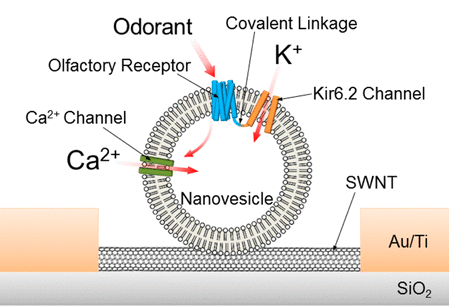
\includegraphics{figures/ch3/ion-channel-nanovesicle-lim2015.png}

}

}

\end{minipage}%
%
\begin{minipage}[t]{0.01\linewidth}

{\centering 

~

}

\end{minipage}%
%
\begin{minipage}[t]{0.03\linewidth}

{\centering 

\raisebox{-\height}{


\includegraphics{figures/(b).png}

}

}

\end{minipage}%
%
\begin{minipage}[t]{0.01\linewidth}

{\centering 

~

}

\end{minipage}%
%
\begin{minipage}[t]{0.45\linewidth}

{\centering 

\raisebox{-\height}{

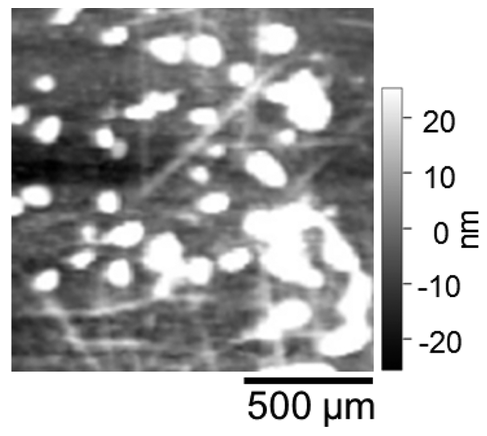
\includegraphics{figures/ch3/afm-nanovesicle-lim2015.png}

}

}

\end{minipage}%
%
\begin{minipage}[t]{0.01\linewidth}

{\centering 

~

}

\end{minipage}%
\newline
\begin{minipage}[t]{0.03\linewidth}

{\centering 

\raisebox{-\height}{


\includegraphics{figures/(c).png}

}

}

\end{minipage}%
%
\begin{minipage}[t]{0.01\linewidth}

{\centering 

~

}

\end{minipage}%
%
\begin{minipage}[t]{0.45\linewidth}

{\centering 

\raisebox{-\height}{

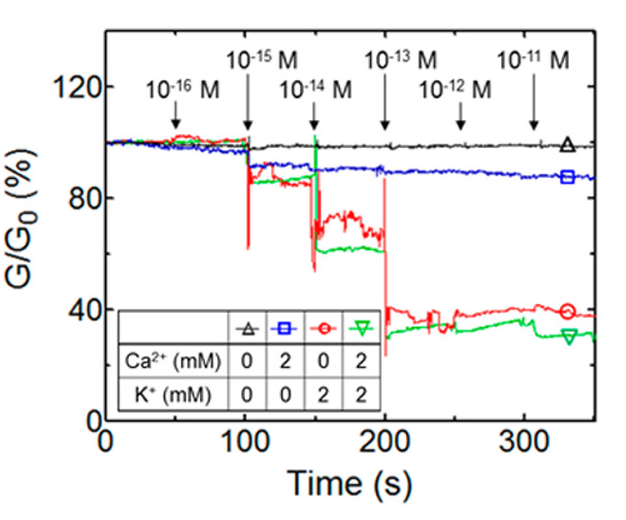
\includegraphics{figures/ch3/nanovesicle-amyl-butyrate-1-lim2015.png}

}

}

\end{minipage}%
%
\begin{minipage}[t]{0.01\linewidth}

{\centering 

~

}

\end{minipage}%
%
\begin{minipage}[t]{0.03\linewidth}

{\centering 

\raisebox{-\height}{

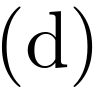
\includegraphics{figures/(d).png}

}

}

\end{minipage}%
%
\begin{minipage}[t]{0.01\linewidth}

{\centering 

~

}

\end{minipage}%
%
\begin{minipage}[t]{0.45\linewidth}

{\centering 

\raisebox{-\height}{

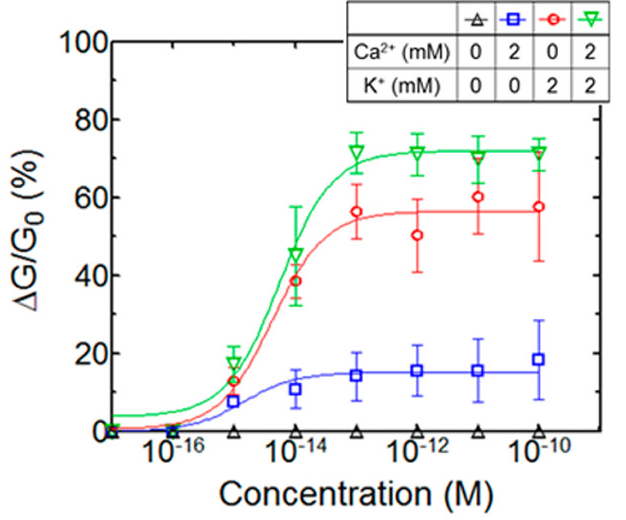
\includegraphics{figures/ch3/nanovesicle-amyl-butyrate-2-lim2015.png}

}

}

\end{minipage}%
%
\begin{minipage}[t]{0.01\linewidth}

{\centering 

~

}

\end{minipage}%

\caption{\label{fig-lim-ion-channel}Schematics detailing the
nanovesicle-based carbon nanotube field-effect biosensor of Lim \emph{et
al.} (a) shows a schematic of the different elements and signalling
pathways present in the sensor, (b) shows an atomic force microscope
image of the functionalised device, (c) shows real-time conductance
changes resulting from amyl butyrate additions to the electrolyte gate
against relevant controls, and (d) shows the dose-dependent response
pattern to amyl butyrate. Reproduced with permission from
\autocite{Lim2015}.}

\end{figure}

Nanovesicle-based odorant receptor biosensors can be used to couple a
vertebrate odorant receptor with an ion channel, where the presence of
analyte leads to a flow of ions into an olfactory cell
\autocite{Lim2015,Dung2018}. Lim \emph{et al.} functionalised a CNT FET
with nanovesicles featuring a human odorant receptor hOR2AG1 covalently
coupled with a potassium ion channel, alongside an endogenous calcium
ion channel, as shown in Figure~\ref{fig-lim-ion-channel} (a). These
nanovesicles were attached to the random carbon nanotube network through
a charge-charge interaction with poly-D-lysine, demonstrated with the
atomic force microscope image shown in Figure~\ref{fig-lim-ion-channel}
(b). Binding of amyl butyrate to hOR2AG1 causes the OR to change
conformation, opening the coupled potassium ion channel and gating the
transistor channel. The real-time signal responses associated with amyl
butyrate binding in the electrolyte environment are shown in
Figure~\ref{fig-lim-ion-channel} (c). Intracellular signalling by the
odorant receptors means that target binding also opens the calcium ion
channel, so a response can be seen when only calcium ions are present.
Without potassium or calcium ions present, ion inflow cannot occur, so
no conductance change is observed. Figure~\ref{fig-lim-ion-channel} (d)
shows the dose dependent response to amyl butyrate in various
electrolytes \autocite{Lim2015}.

\begin{figure}

\begin{minipage}[t]{0.03\linewidth}

{\centering 

\raisebox{-\height}{


\includegraphics{figures/(a).png}

}

}

\end{minipage}%
%
\begin{minipage}[t]{0.04\linewidth}

{\centering 

~

}

\end{minipage}%
%
\begin{minipage}[t]{0.90\linewidth}

{\centering 

\raisebox{-\height}{

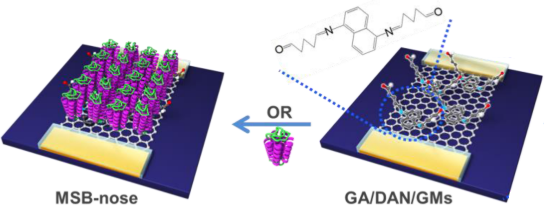
\includegraphics{figures/ch3/kwon2015-OR-graphene.png}

}

}

\end{minipage}%
%
\begin{minipage}[t]{0.04\linewidth}

{\centering 

~

}

\end{minipage}%
\newline
\begin{minipage}[t]{0.03\linewidth}

{\centering 

\raisebox{-\height}{


\includegraphics{figures/(b).png}

}

}

\end{minipage}%
%
\begin{minipage}[t]{0.01\linewidth}

{\centering 

~

}

\end{minipage}%
%
\begin{minipage}[t]{0.45\linewidth}

{\centering 

\raisebox{-\height}{

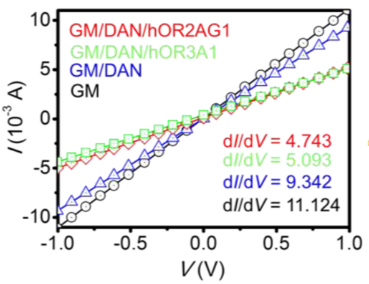
\includegraphics{figures/ch3/kwon2015_transfer.png}

}

}

\end{minipage}%
%
\begin{minipage}[t]{0.01\linewidth}

{\centering 

~

}

\end{minipage}%
%
\begin{minipage}[t]{0.03\linewidth}

{\centering 

\raisebox{-\height}{


\includegraphics{figures/(c).png}

}

}

\end{minipage}%
%
\begin{minipage}[t]{0.01\linewidth}

{\centering 

~

}

\end{minipage}%
%
\begin{minipage}[t]{0.45\linewidth}

{\centering 

\raisebox{-\height}{

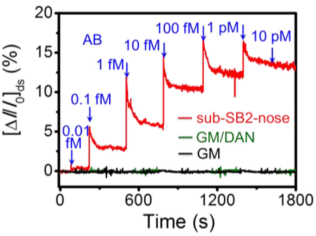
\includegraphics{figures/ch3/kwon2015-amyl-butyrate.png}

}

}

\end{minipage}%
%
\begin{minipage}[t]{0.01\linewidth}

{\centering 

~

}

\end{minipage}%
\newline
\begin{minipage}[t]{0.03\linewidth}

{\centering 

\raisebox{-\height}{

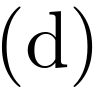
\includegraphics{figures/(d).png}

}

}

\end{minipage}%
%
\begin{minipage}[t]{0.01\linewidth}

{\centering 

~

}

\end{minipage}%
%
\begin{minipage}[t]{0.45\linewidth}

{\centering 

\raisebox{-\height}{

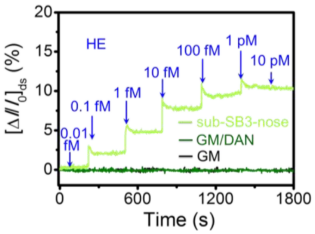
\includegraphics{figures/ch3/kwon2015-helional.png}

}

}

\end{minipage}%
%
\begin{minipage}[t]{0.01\linewidth}

{\centering 

~

}

\end{minipage}%
%
\begin{minipage}[t]{0.03\linewidth}

{\centering 

\raisebox{-\height}{


\includegraphics{figures/(e).png}

}

}

\end{minipage}%
%
\begin{minipage}[t]{0.01\linewidth}

{\centering 

~

}

\end{minipage}%
%
\begin{minipage}[t]{0.45\linewidth}

{\centering 

\raisebox{-\height}{

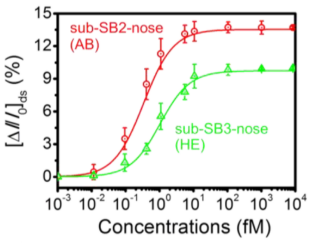
\includegraphics{figures/ch3/kwon2015-dose.png}

}

}

\end{minipage}%
%
\begin{minipage}[t]{0.01\linewidth}

{\centering 

~

}

\end{minipage}%

\caption{\label{fig-kwon-multiplexed}Schematics showing the odorant
receptor-functionalised graphene field-effect biosensor of Kwon \emph{et
al.} (a) shows the functionalisation of odorant receptors onto graphene
using non-covalently attached GA-modified DAN linker; (b) compares
transfer characteristics of the device with graphene only (GM), graphene
with DAN linker (GM/DAN), and after modification with one of two
different ORs (hOR2AG1, hOR3A1); (c) shows the real-time responses of
the liquid-gated hOR2AG1-modified transistor (sub-SB2) to various
concentrations of amyl butyrate (AB) analyte; (d) shows the real-time
responses of the hOR3A1-modified transistor (sub-SB3) to various
concentrations of helional (HE) analyte; and (e) shows the
dose-dependent response curve corresponding to the sub-SB2 and sub-SB3
sensors. Reproduced with permission from \autocite{Kwon2015}.}

\end{figure}

Odorant receptors can also be expressed in the native cell membrane and
attached directly to the biosensor channel. Here, the changes in odorant
receptor conformation that result from analyte binding cause affects the
distance between charges on the odorant receptor and the transducer
channel, gating the channel \autocite{Kwon2015,Dung2018}. Kwon \emph{et
al.} functionalised graphene field-effect transistors with human odorant
receptors hOR2AG1 and hOR3A1 using non-covalently attached
1,5-diaminonaphthalene (DAN) modified with glutaraldehyde (GA) as a
linker, as shown in Figure~\ref{fig-kwon-multiplexed} (a). The odorant
receptors attach to the GA-modified DAN via a Schiff-base reaction
\autocite{Subasi2022}. OR attachment was demonstrated by SEM imaging as
well as a significant change in device resistance, shown in
Figure~\ref{fig-kwon-multiplexed} (b). Both hOR2AG1 and hOR3A1 showed
real-time responses to their corresponding target analyte at
sub-femtomolar concentrations, as shown in
Figure~\ref{fig-kwon-multiplexed} (c) and
Figure~\ref{fig-kwon-multiplexed} (d) respectively. No responses were
seen from linker-modified graphene to the same analyte additions. The
dose-dependent response curve of both these odorant receptor sensors is
shown in Figure~\ref{fig-kwon-multiplexed} (e). As in
Figure~\ref{fig-lim-ion-channel} (d), a Langmuir-type dose response
behaviour was seen, where a logarithmic increase in signal response is
observed for sub-femtomolar or femtomolar concentration analyte
additions, which gives way to saturation behaviour with picomolar
additions.

\begin{figure}

\begin{minipage}[t]{0.03\linewidth}

{\centering 

\raisebox{-\height}{


\includegraphics{figures/(a).png}

}

}

\end{minipage}%
%
\begin{minipage}[t]{0.01\linewidth}

{\centering 

~

}

\end{minipage}%
%
\begin{minipage}[t]{0.45\linewidth}

{\centering 

\raisebox{-\height}{

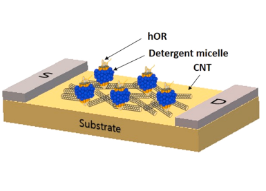
\includegraphics{figures/ch3/yoo2022-micelle-cnt.png}

}

}

\end{minipage}%
%
\begin{minipage}[t]{0.01\linewidth}

{\centering 

~

}

\end{minipage}%
%
\begin{minipage}[t]{0.03\linewidth}

{\centering 

\raisebox{-\height}{


\includegraphics{figures/(b).png}

}

}

\end{minipage}%
%
\begin{minipage}[t]{0.01\linewidth}

{\centering 

~

}

\end{minipage}%
%
\begin{minipage}[t]{0.45\linewidth}

{\centering 

\raisebox{-\height}{

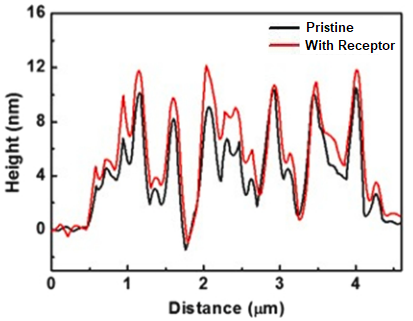
\includegraphics{figures/ch3/yoo2022-AFM.png}

}

}

\end{minipage}%
%
\begin{minipage}[t]{0.01\linewidth}

{\centering 

~

}

\end{minipage}%
\newline
\begin{minipage}[t]{0.03\linewidth}

{\centering 

\raisebox{-\height}{


\includegraphics{figures/(c).png}

}

}

\end{minipage}%
%
\begin{minipage}[t]{0.01\linewidth}

{\centering 

~

}

\end{minipage}%
%
\begin{minipage}[t]{0.45\linewidth}

{\centering 

\raisebox{-\height}{

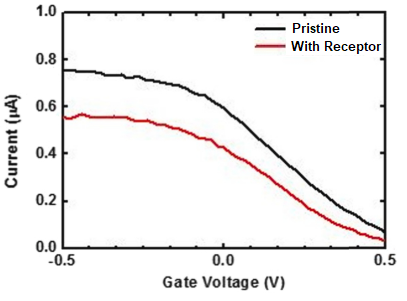
\includegraphics{figures/ch3/yoo2022-TX.png}

}

}

\end{minipage}%
%
\begin{minipage}[t]{0.01\linewidth}

{\centering 

~

}

\end{minipage}%
%
\begin{minipage}[t]{0.03\linewidth}

{\centering 

\raisebox{-\height}{

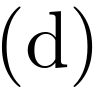
\includegraphics{figures/(d).png}

}

}

\end{minipage}%
%
\begin{minipage}[t]{0.01\linewidth}

{\centering 

~

}

\end{minipage}%
%
\begin{minipage}[t]{0.45\linewidth}

{\centering 

\raisebox{-\height}{

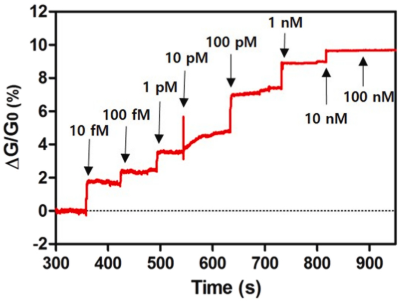
\includegraphics{figures/ch3/yoo2022-DMMP.png}

}

}

\end{minipage}%
%
\begin{minipage}[t]{0.01\linewidth}

{\centering 

~

}

\end{minipage}%
\newline
\begin{minipage}[t]{0.03\linewidth}

{\centering 

\raisebox{-\height}{


\includegraphics{figures/(e).png}

}

}

\end{minipage}%
%
\begin{minipage}[t]{0.01\linewidth}

{\centering 

~

}

\end{minipage}%
%
\begin{minipage}[t]{0.45\linewidth}

{\centering 

\raisebox{-\height}{

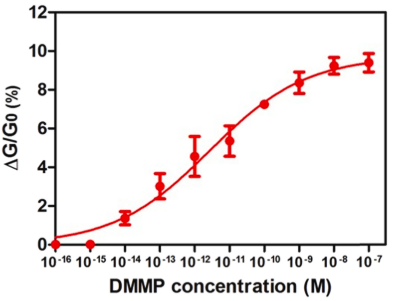
\includegraphics{figures/ch3/yoo2022-DMMP-2.png}

}

}

\end{minipage}%
%
\begin{minipage}[t]{0.01\linewidth}

{\centering 

~

}

\end{minipage}%
%
\begin{minipage}[t]{0.03\linewidth}

{\centering 

\raisebox{-\height}{


\includegraphics{figures/(f).png}

}

}

\end{minipage}%
%
\begin{minipage}[t]{0.01\linewidth}

{\centering 

~

}

\end{minipage}%
%
\begin{minipage}[t]{0.45\linewidth}

{\centering 

\raisebox{-\height}{

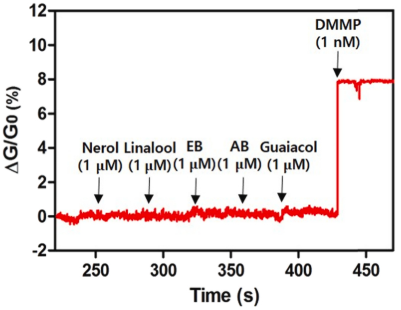
\includegraphics{figures/ch3/yoo2022-DMMP-3.png}

}

}

\end{minipage}%
%
\begin{minipage}[t]{0.01\linewidth}

{\centering 

~

}

\end{minipage}%

\caption{\label{fig-yoo-micelle}Schematics of the micelle-based carbon
nanotube field-effect transistor of Yoo \emph{et al.} (a) shows the
functionalisation of detergent micelles onto the carbon nanotube network
channel; (b) shows the same height profile across an atomic force
microscope image of the carbon nanotube network before and after
functionalisation with micelles using PBASE; (c) shows the liquid-gated
transfer characteristic of a device channel before and after
functionalisation with PBASE and micelles; (d) shows real-time responses
of the functionalised, liquid-gated channel to additions of dimethyl
methylphosphonate (DMMP) analyte; (e) shows the dose-dependent response
curve to DMMP; and (f) shows a control series demonstrating the
selective behaviour of the sensor, where EB is ethyl butyrate and AB is
amyl butyrate. Reproduced with permission from \autocite{Yoo2022}.}

\end{figure}

Biosensors have also been produced where odorant receptors are held in a
detergent micelle format instead of the native cell membrane. The
mechanism behind sensing is the same as for odorant receptors in the
cell membrane, where a conformational change in the odorant receptors
leads to channel gating \autocite{Dung2018,Yoo2022}. Yoo \emph{et al.}
functionalised random-network CNT FETs with detergent micelles which
contained human odorant receptor hOR2T7. PBASE was used as the linker
molecule, which attaches to the odorant receptor via its amine group and
non-covalently tethers it to the transducer, illustrated in
Figure~\ref{fig-yoo-micelle} (a). Successful immobilisation was
demonstrated by a raised atomic force microscope height profile after
receptor attachment (Figure~\ref{fig-yoo-micelle} (b)) and an on-current
drop in the liquid-gated transfer characteristics of the device
(Figure~\ref{fig-yoo-micelle} (c)). The sensor showed sharp real-time
responses to the addition of DMMP concentrations, as seen in
Figure~\ref{fig-yoo-micelle} (d). The dose dependence curve for DMMP
responses is shown in in Figure~\ref{fig-yoo-micelle} (e), again showing
a Langmuir-type response curve to successive DMMP additions. Various
analytes with a similar scent to DMMP were added at high concentrations
to the liquid-gate, shown in Figure~\ref{fig-yoo-micelle} (f). No
response was seen to any these additions, demonstrating the selectivity
of the sensor.

In the first study of this kind, Goldsmith \emph{et al.} demonstrated
that a single-CNT device functionalised with mOR174-9 odorant receptors
in either a micelle or nanodisc format could be used as a vapour-phase
biosensor. Micelle immobilisation was confirmed using atomic force
microscopy, as shown in Figure~\ref{fig-eugenol-responses} (a). The mOR
CNT FETs were exposed to nitrogen flow at 50\% relative humidity. The
conductance across the channel was measured while a specific
concentration of the positive ligand eugenol was added to the constant
flow for 100 s, then removed from the flow for 100 s. This cycle was
repeated five times. Figure~\ref{fig-eugenol-responses} (b) shows that
significant real-time current increases of up to \(\sim\) 9\% were
observed during each cycle of exposure to eugenol. The device still
responded to eugenol cycles after 69 days of storage in 25\% (v/v)
ethanol at 4°C. This persistent activity may result from the long-lived
nanodisc format used \autocite{Goldsmith2011}. As far as the author
knows, no investigation up until now has investigated whether this
behaviour can be replicated for insect odorant receptor devices. It is
not clear that the vertebrate odorant receptors used here can simply be
substituted for iORs for vapour-phase sensing. The difference between
receptors is discussed further in the subsequent section.

\begin{figure}

\begin{minipage}[t]{0.03\linewidth}

{\centering 

\raisebox{-\height}{


\includegraphics{figures/(a).png}

}

}

\end{minipage}%
%
\begin{minipage}[t]{0.01\linewidth}

{\centering 

~

}

\end{minipage}%
%
\begin{minipage}[t]{0.40\linewidth}

{\centering 

\raisebox{-\height}{

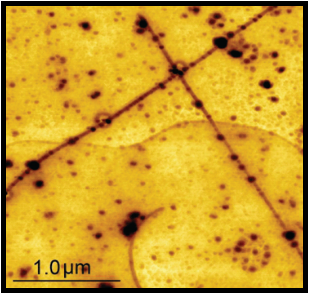
\includegraphics{figures/ch3/afm-nanodisc-goldsmith.png}

}

}

\end{minipage}%
%
\begin{minipage}[t]{0.01\linewidth}

{\centering 

~

}

\end{minipage}%
%
\begin{minipage}[t]{0.03\linewidth}

{\centering 

\raisebox{-\height}{


\includegraphics{figures/(b).png}

}

}

\end{minipage}%
%
\begin{minipage}[t]{0.01\linewidth}

{\centering 

~

}

\end{minipage}%
%
\begin{minipage}[t]{0.50\linewidth}

{\centering 

\raisebox{-\height}{

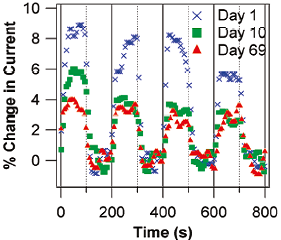
\includegraphics{figures/ch3/eugenol-goldsmith.png}

}

}

\end{minipage}%
%
\begin{minipage}[t]{0.01\linewidth}

{\centering 

~

}

\end{minipage}%

\caption{\label{fig-eugenol-responses}The functionalisation of mOR174-9
nanodiscs onto single-CNT field effect transistor vapour sensing use is
demonstrated with an atomic force microscope image in (a), while (b)
shows real-time responses of the sensor to 2 ppm eugenol vapour. The
response to eugenol on day 69 (red triangles) indicates that the device
retains the ability to respond to eugenol 10 weeks after
functionalisation. Reproduced with permission from
\autocite{Goldsmith2011}.}

\end{figure}

\hypertarget{sec-insect-OR-biosensors}{%
\section{Insect Odorant Receptor Field-Effect Transistor
Biosensors}\label{sec-insect-OR-biosensors}}

\hypertarget{insect-odorant-receptors}{%
\subsection{Insect Odorant Receptors}\label{insect-odorant-receptors}}

Insect odorant (or olfactory) receptors (iORs) are a diverse range of
odorant-sensitive seven-transmembrane proteins located in the dendrite
cells of insect sensory hairs, known as sensilla
\autocite{Clyne1999,Carraher2015,Brito2016,Wicher2021}. When volatile
compounds enter the sensilla, they are carried by odorant binding
proteins (OBPs) through an aqueous environment to the dendrite cells
\autocite{Carraher2015,Brito2016,Wicher2021}. These cells possess a
insect-specific set of `tuning' iORs alongside a generic co-receptor
known as `ORCO' (Odorant Receptor Co-Receptor)
\autocite{Carraher2015,Butterwick2018,Khadka2019,Wicher2021}. The ORCO
co-receptor is insensitive to target compounds (aside from synthetic
compounds like VUAA1). Instead, it couples with the tuning iOR to form a
non-selective, permeable ion channel
\autocite{Butterwick2018,Wicher2021}. When a compound binds to a tuning
iOR, the ion channel opens to allow cations to travel across the cell
membrane, activating intracellular signalling
\autocite{Smart2008,Wicher2008,Sato2008,Carraher2015,Brito2016,Butterwick2018,Wicher2021}.
The combination of resulting OR signals is sent to the insect brain for
interpretation as an odor. The tuning iORs respond to (or are inhibited
by) a huge variety of odors
\autocite{Hallem2004,Carraher2015,Wicher2021}. A database describing the
various odorant receptors of \emph{Drosophilia melanogaster} and their
corresponding target analytes can be consulted online
\autocite{Munch2016}.

\begin{figure}

{\centering 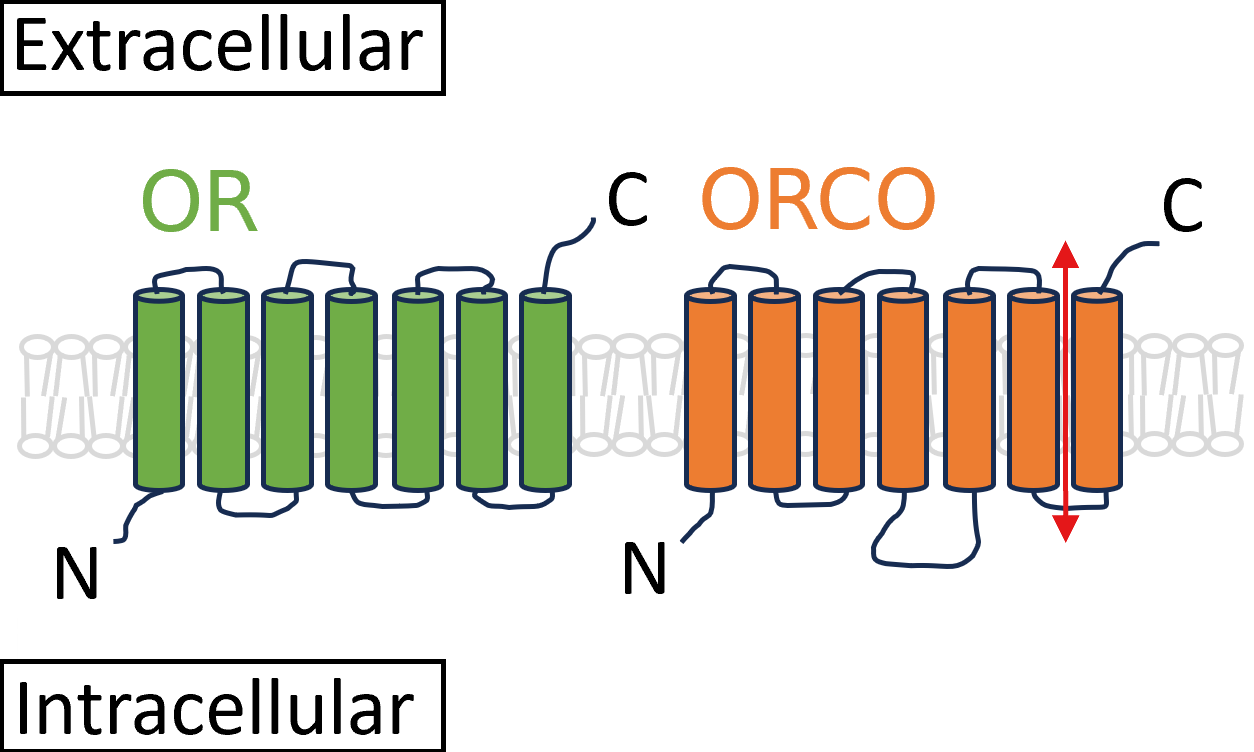
\includegraphics[width=0.55\textwidth,height=\textheight]{figures/ch3/OR_diagram.png}

}

\caption{\label{fig-iOR-membrane}The tuning OR and odorant receptor
coreceptor (ORCO) on the native cell membrane, with C-terminus and
N-terminus indicated. The red arrow indicates the location of ion
transport across the membrane. Adapted from
\autocite{Brito2016,Wicher2021}.}

\end{figure}

Vertebrate odorant receptor proteins are terminated with an amine group
outside the cell membrane, known as the N-terminus, and terminated with
a carboxyl group inside the cell membrane, known as the C-terminus.
Initially, iORs were thought to be similar in structure to vertebrate
GPCRs \autocite{Clyne1999}, but is now known that iORs have a completely
different topology and mechanism, despite also being a
seven-transmembrane protein. The terminus configuration is inverted: the
C-terminus of the iOR is extracellular, and the N-terminus is
intracellular
\autocite{Smart2008,Glatz2011,Carraher2015,Brito2016,Wicher2021}.
Furthermore, there is no sequence similarity between iORs and GPCRs.
Evolutionarily, insect odorant receptors are thought to be closely
related to insect gustatory receptors (GRs), while they bear no relation
to GPCRs \autocite{Glatz2011,Carraher2015,Wicher2021}. However, despite
iORs not being GPCRs, some interaction between the iOR complex and the
G-protein of the olfactory cell plays a role in odor detection \emph{in
vivo} \autocite{Wicher2008,Wicher2021}. The \emph{in vivo} configuration
of the odorant receptor on the cell membrane, showing the terminus
configuration and location of ORCO ion channel, is illustrated in
Figure~\ref{fig-iOR-membrane}.

\hypertarget{sensor-functionalisation}{%
\subsection{Sensor Functionalisation}\label{sensor-functionalisation}}

\begin{figure}

\begin{minipage}[t]{0.03\linewidth}

{\centering 

\raisebox{-\height}{


\includegraphics{figures/(a).png}

}

}

\end{minipage}%
%
\begin{minipage}[t]{0.01\linewidth}

{\centering 

~

}

\end{minipage}%
%
\begin{minipage}[t]{0.45\linewidth}

{\centering 

\raisebox{-\height}{

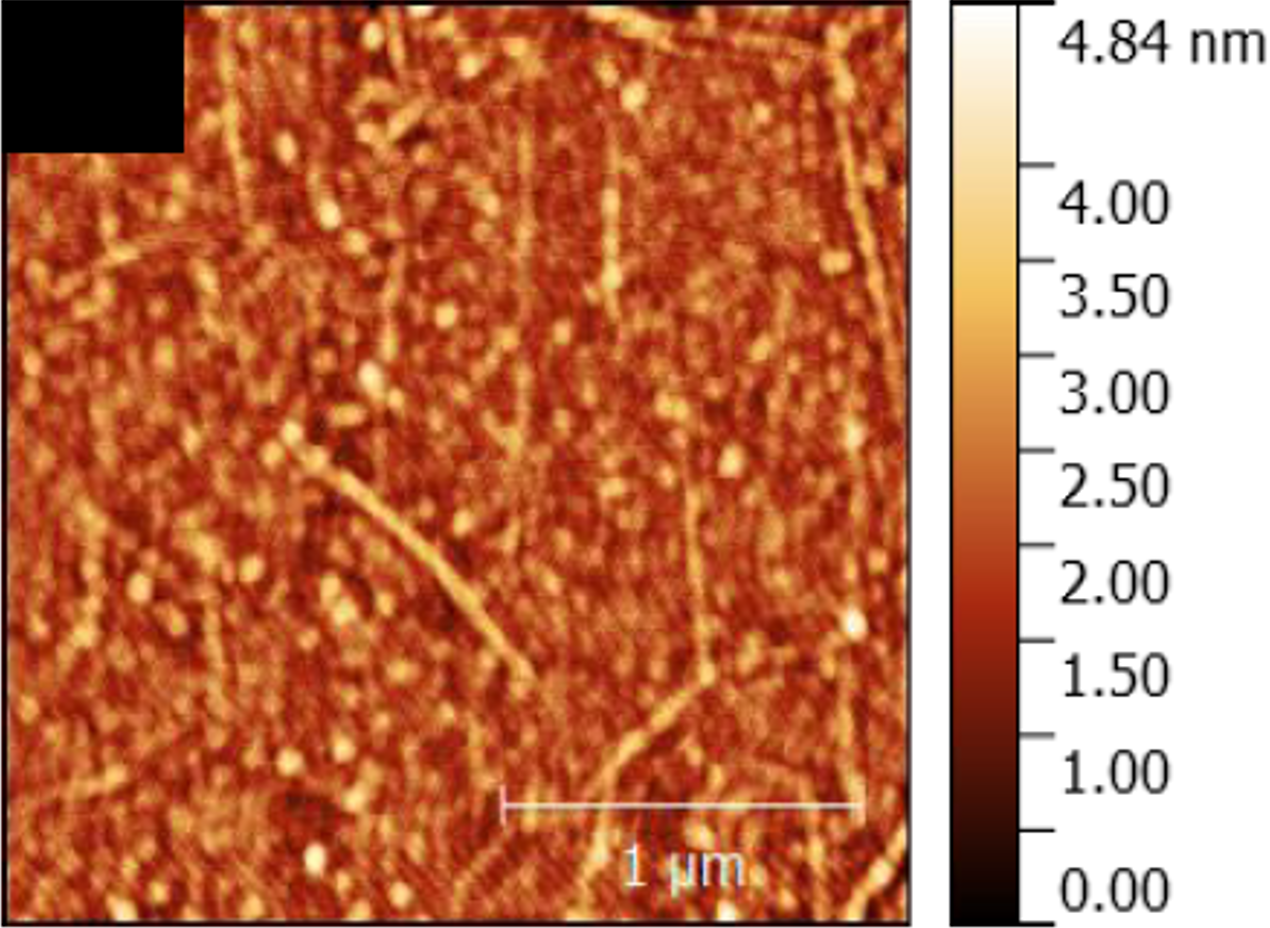
\includegraphics{figures/ch3/pristine_graphene_murugathas.png}

}

}

\end{minipage}%
%
\begin{minipage}[t]{0.01\linewidth}

{\centering 

~

}

\end{minipage}%
%
\begin{minipage}[t]{0.03\linewidth}

{\centering 

\raisebox{-\height}{


\includegraphics{figures/(b).png}

}

}

\end{minipage}%
%
\begin{minipage}[t]{0.01\linewidth}

{\centering 

~

}

\end{minipage}%
%
\begin{minipage}[t]{0.45\linewidth}

{\centering 

\raisebox{-\height}{

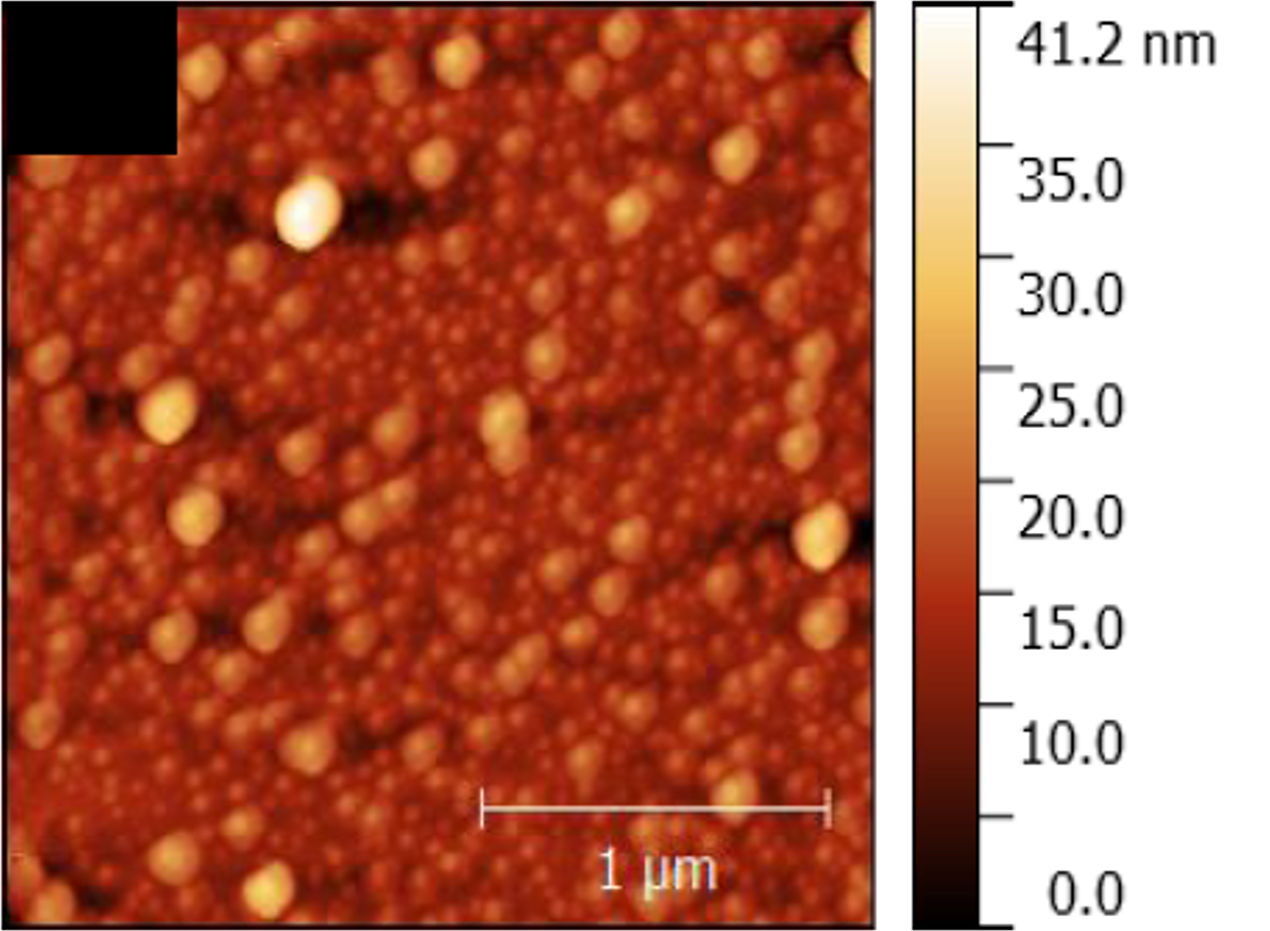
\includegraphics{figures/ch3/OR22a_graphene_murugathas.png}

}

}

\end{minipage}%
%
\begin{minipage}[t]{0.01\linewidth}

{\centering 

~

}

\end{minipage}%
\newline
\begin{minipage}[t]{0.03\linewidth}

{\centering 

\raisebox{-\height}{


\includegraphics{figures/(c).png}

}

}

\end{minipage}%
%
\begin{minipage}[t]{0.01\linewidth}

{\centering 

~

}

\end{minipage}%
%
\begin{minipage}[t]{0.45\linewidth}

{\centering 

\raisebox{-\height}{

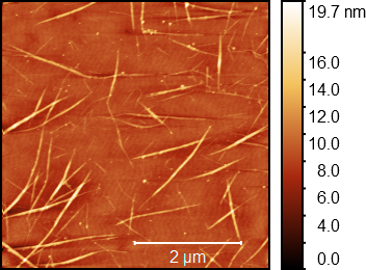
\includegraphics{figures/ch3/pristine_CNT_murugathas.png}

}

}

\end{minipage}%
%
\begin{minipage}[t]{0.01\linewidth}

{\centering 

~

}

\end{minipage}%
%
\begin{minipage}[t]{0.03\linewidth}

{\centering 

\raisebox{-\height}{

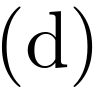
\includegraphics{figures/(d).png}

}

}

\end{minipage}%
%
\begin{minipage}[t]{0.01\linewidth}

{\centering 

~

}

\end{minipage}%
%
\begin{minipage}[t]{0.45\linewidth}

{\centering 

\raisebox{-\height}{

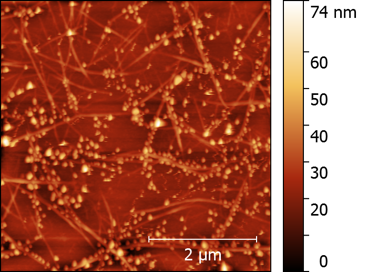
\includegraphics{figures/ch3/OR22a_CNT_murugathas.png}

}

}

\end{minipage}%
%
\begin{minipage}[t]{0.01\linewidth}

{\centering 

~

}

\end{minipage}%

\caption{\label{fig-functionalisation-AFM-literature}Atomic force
microscope images of (a) a pristine graphene monolayer, (b) a OR22a
nanodisc-functionalised graphene monolayer, (c) a pristine carbon
nanotube network, and (d) an OR22a nanodisc-functionalised carbon
nanotube network. Reproduced with permission from
\autocite{Murugathas2019a,Murugathas2020}.}

\end{figure}

Murugathas \emph{et al.} attached a variety of insect odorant receptors
to carbon nanotubes and graphene field-effect transistors using a
nanodisc format. Atomic force microscope images of a graphene monolayer
before and after immobilisation of OR22a nanodiscs with PBASE linker are
shown in Figure~\ref{fig-functionalisation-AFM-literature} (a) and (b)
respectively, while atomic force microscope images of a randomly
deposited carbon nanotube network before and after OR22a nanodisc
immobilisation with PBASE are shown in
Figure~\ref{fig-functionalisation-AFM-literature} (c) and (d)
respectively. Features are seen across the surface of the
post-functionalisation image which are tens of nanometers in height. On
the nanotube network, these features are seen directly next to nanotube
bundles, indicating selective attachment to the nanotubes over the
silicon dioxide substrate. As nanodiscs are only 10-20 nm in height, it
appears that these features are large agglomerates of nanodiscs
\autocite{Nath2007,Bayburt2010,Murugathas2019a,Murugathas2020}. As seen
previously for a carbon nanotube network FET in
Section~\ref{sec-odorant-receptors-biosensors}, functionalisation occurs
by non-covalent attachment of PBASE to the channel, and covalent
attachment of the PBASE linker to the odorant receptor amine group. The
nanodisc membrane also possesses amine residues \autocite{Bayburt2010},
so in some cases immobilisation may be directly between the PBASE linker
and nanodisc membrane.

\begin{figure}

\begin{minipage}[t]{0.03\linewidth}

{\centering 

\raisebox{-\height}{


\includegraphics{figures/(a).png}

}

}

\end{minipage}%
%
\begin{minipage}[t]{0.01\linewidth}

{\centering 

~

}

\end{minipage}%
%
\begin{minipage}[t]{0.45\linewidth}

{\centering 

\raisebox{-\height}{

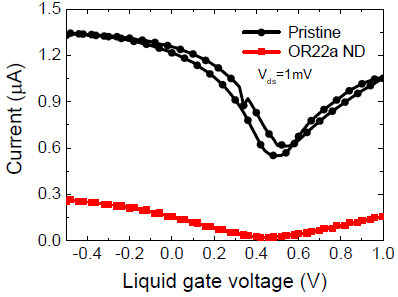
\includegraphics{figures/ch3/OR22a_ND_GFET.png}

}

}

\end{minipage}%
%
\begin{minipage}[t]{0.01\linewidth}

{\centering 

~

}

\end{minipage}%
%
\begin{minipage}[t]{0.03\linewidth}

{\centering 

\raisebox{-\height}{


\includegraphics{figures/(b).png}

}

}

\end{minipage}%
%
\begin{minipage}[t]{0.01\linewidth}

{\centering 

~

}

\end{minipage}%
%
\begin{minipage}[t]{0.45\linewidth}

{\centering 

\raisebox{-\height}{

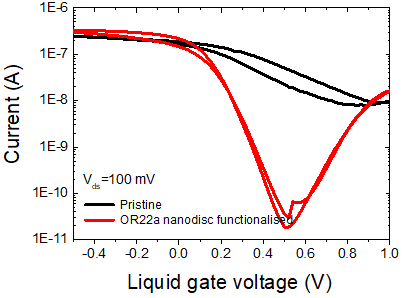
\includegraphics{figures/ch3/OR22a_ND_CNTFET.png}

}

}

\end{minipage}%
%
\begin{minipage}[t]{0.01\linewidth}

{\centering 

~

}

\end{minipage}%
\newline
\begin{minipage}[t]{0.03\linewidth}

{\centering 

\raisebox{-\height}{

\includegraphics{figures/(c).png}

}

}

\end{minipage}%
%
\begin{minipage}[t]{0.01\linewidth}

{\centering 

~

}

\end{minipage}%
%
\begin{minipage}[t]{0.45\linewidth}

{\centering 

\raisebox{-\height}{

\includegraphics{figures/ch3/Empty_ND_GFET.png}

}

}

\end{minipage}%
%
\begin{minipage}[t]{0.01\linewidth}

{\centering 

~

}

\end{minipage}%
%
\begin{minipage}[t]{0.03\linewidth}

{\centering 

\raisebox{-\height}{

\includegraphics{figures/(d).png}

}

}

\end{minipage}%
%
\begin{minipage}[t]{0.01\linewidth}

{\centering 

~

}

\end{minipage}%
%
\begin{minipage}[t]{0.45\linewidth}

{\centering 

\raisebox{-\height}{

\includegraphics{figures/ch3/Empty_ND_CNTFET.png}

}

}

\end{minipage}%
%
\begin{minipage}[t]{0.01\linewidth}

{\centering 

~

}

\end{minipage}%

\caption{\label{fig-functionalisation-literature}Transfer characteristic
curves before and after functionalisation of (a) an OR22a
nanodisc-functionalised graphene FET, (b) an OR22a
nanodisc-functionalised CNT network FET, (c) an empty
nanodisc-functionalised graphene FET and (d) an empty
nanodisc-functionalised CNT network FET. Reproduced with permission from
\autocite{Murugathas2019a,Murugathas2020}.}

\end{figure}

Functionalisation of a FET device channel with iORs significantly alters
the transfer characteristics of that channel. Murugathas \emph{et al.}
found that successful functionalisation of a CNT FET device with iORs
would typically increase the device on-current, increase its on-off
ratio and cause a significant negative shift in threshold voltage, as
shown in Figure~\ref{fig-functionalisation-literature} (a)
\autocite{Murugathas2019a}. Meanwhile, successful functionalisation of a
graphene device with iORs would typically dramatically decrease the
device on-current and cause a negative shift in Dirac voltage, as seen
in Figure~\ref{fig-functionalisation-literature} (b)
\autocite{Murugathas2020}. These changes are not simply the result of
linker attachment to the channel surface \autocite{Murugathas2019a}. It
is thought that the negative shift of both threshold and Dirac voltages
are caused by the N-terminus amine groups on the odorant receptors or
amine groups on the nanodisc membrane scaffold proteins donating
electrons to the device channel, which has a similar effect to doping
the channel with impurities
\autocite{Bradley2004,Murugathas2019a,Murugathas2020}. Note that very
similar changes occur when functionalising with empty nanodiscs which
contain no odorant receptors, shown in
Figure~\ref{fig-functionalisation-literature} (c) and
Figure~\ref{fig-functionalisation-literature} (d). Unless the odorant
receptors attach preferentially to the network over nanodiscs, it
appears the gating effect is predominantly due to the large-scale
attachment of nanodisc membranes.

\hypertarget{sensing-behaviour}{%
\subsection{Sensing Behaviour}\label{sensing-behaviour}}

\begin{figure}

\begin{minipage}[t]{0.03\linewidth}

{\centering 

\raisebox{-\height}{

\includegraphics{figures/(a).png}

}

}

\end{minipage}%
%
\begin{minipage}[t]{0.01\linewidth}

{\centering 

~

}

\end{minipage}%
%
\begin{minipage}[t]{0.45\linewidth}

{\centering 

\raisebox{-\height}{

\includegraphics{figures/ch3/OR22a_realtime_normalised_CNTFET_1.png}

}

}

\end{minipage}%
%
\begin{minipage}[t]{0.01\linewidth}

{\centering 

~

}

\end{minipage}%
%
\begin{minipage}[t]{0.03\linewidth}

{\centering 

\raisebox{-\height}{

\includegraphics{figures/(b).png}

}

}

\end{minipage}%
%
\begin{minipage}[t]{0.01\linewidth}

{\centering 

~

}

\end{minipage}%
%
\begin{minipage}[t]{0.45\linewidth}

{\centering 

\raisebox{-\height}{

\includegraphics{figures/ch3/OR22a_realtime_normalised_GFET_1.png}

}

}

\end{minipage}%
%
\begin{minipage}[t]{0.01\linewidth}

{\centering 

~

}

\end{minipage}%
\newline
\begin{minipage}[t]{0.03\linewidth}

{\centering 

\raisebox{-\height}{

\includegraphics{figures/(c).png}

}

}

\end{minipage}%
%
\begin{minipage}[t]{0.01\linewidth}

{\centering 

~

}

\end{minipage}%
%
\begin{minipage}[t]{0.45\linewidth}

{\centering 

\raisebox{-\height}{

\includegraphics{figures/ch3/OR22a_realtime_normalised_CNTFET_2.png}

}

}

\end{minipage}%
%
\begin{minipage}[t]{0.01\linewidth}

{\centering 

~

}

\end{minipage}%
%
\begin{minipage}[t]{0.03\linewidth}

{\centering 

\raisebox{-\height}{

\includegraphics{figures/(d).png}

}

}

\end{minipage}%
%
\begin{minipage}[t]{0.01\linewidth}

{\centering 

~

}

\end{minipage}%
%
\begin{minipage}[t]{0.45\linewidth}

{\centering 

\raisebox{-\height}{

\includegraphics{figures/ch3/OR22a_realtime_normalised_GFET_2.png}

}

}

\end{minipage}%
%
\begin{minipage}[t]{0.01\linewidth}

{\centering 

~

}

\end{minipage}%

\caption{\label{fig-iOR-sensing-literature}Real-time responses to
concentrations of methyl hexanoate in \(1 \times\) phosphate buffer
saline (PBS) with 1\% v/v DMSO by (a) an OR22a nanodisc-functionalised
CNT network FET and (b) an OR22a nanodisc-functionalised graphene FET,
alongside the normalised signal response curves corresponding to (c) CNT
network FETs and (d) graphene FETs. The response curves show the
cumulative responses of OR22a-functionalised devices to both the
positive ligand methyl hexanoate (green) and negative ligand
\emph{trans}-2-hexan-1-al (black). They also show the cumulative
response of a empty nanodisc functionalised device to methyl hexanoate
(purple). Reproduced with permission from
\autocite{Murugathas2019a,Murugathas2020}.}

\end{figure}

Figure~\ref{fig-iOR-sensing-literature} (a) and (b) show the respective
responses of the OR22a-functionalised CNT FET and graphene FET to
various concentrations of methyl hexanoate in real-time. This result
demonstrates that iOR-FETs are sensitive down to the femtomolar scale in
an aqueous environment. Figure~\ref{fig-iOR-sensing-literature} (c) and
(d) compares the dose dependent responses to methyl hexanoate from
multiple OR22a-functionalised devices to that of relevant controls. It
was verified that the OR22a-functionalised devices would not respond to
\emph{trans}-2-hexan-1-al, the negative ligand for OR22a; it was also
verified that empty nanodiscs would not respond non-selectively to the
positive ligand \autocite{Murugathas2019a,Murugathas2020}. It is notable
that unlike iORs \emph{in vivo}, ORCO does not appear to be required for
the bioelectronic nose to function
\autocite{Murugathas2019a,Murugathas2020,Khadka2019,Cheema2021}.
Furthermore, G-protein signaling pathways are not required
\autocite{Sato2014}. It has been proposed that the signal response
results from the positive ligand binding to the iOR protein, causing a
change in conformation, the same mechanism underpinning the behaviour of
many of the vertebrate odorant receptor sensors seen in
Section~\ref{sec-odorant-receptors-biosensors}. Cheema \emph{et al.}
used neutron reflectometry to demonstrate that OR22a nanodiscs undergo a
1 nm height change after ethyl hexanoate exposure, likely resulting from
a structural change \autocite{Cheema2021}.

This change most likely affects the channel in one of two ways. The
first involves transfer of charge from the iOR to the channel, reducing
I\(_{d}\) and causing a negative threshold voltage (or Dirac point)
shift. Another could be a more indirect electrostatic gating effect from
movement of charge within the Debye screening length of the channel. The
Debye length of \(1 \times\) PBS buffer is typically much shorter than
the height of a single nanodisc \autocite{Murugathas2019a}. However, if
structural changes in the iOR were primarily occurring at its base, it
is still possible that the electrostatic gating could be the primary
sensing mechanism. From further development and examination of iOR-based
biosensors, new insights into the mechanisms underlying the nanodisc
signal transduction may emerge \autocite{Glatz2011}. As discussed here,
the literature has primarily focused on the operation of iOR carbon
nanotube and graphene FET biosensors in an aqueous environment
\autocite{Murugathas2019a,Murugathas2020}. It is as yet unknown whether
insect odorant receptors can operate in a vapour-phase environment, but
this possibility is explored in this thesis.

\hypertarget{sec-non-specific-binding}{%
\section{Non-Specific Binding}\label{sec-non-specific-binding}}

Non-specific binding (NSB) refers to any attachment within the sensing
environment not related to the specific analyte of interest
\autocite{Lichtenberg2019,Shkodra2021}. Non-specific binding is
particularly significant for protein-functionalised devices. Proteins
may be spontaneously adsorbed onto carbon nanotube or graphene surfaces
during functionalisation in a manner which is not linker-mediated
\autocite{Bradley2004,Star2003a,Chen2004}. Non-covalently bound proteins
may detach and reattach to available surfaces in a non-specific manner
when exposed to a high ionic strength electrolyte post-functionalisation
\autocite{Dung2018}. Non-specific binding may also result from
protein-protein interactions, misoriented attachment of proteins,
attachment to a sticky substrate \autocite{Chen2004,Lichtenberg2019}. It
can also result from electrostatic binding to any charged surface
present, such as the gold electrodes \autocite{Garcia-Aljaro2010} or
Ag/AgCl reference electrode
\autocite{Chen2004,Minot2007,Lichtenberg2019}. Liquid-gated graphene and
carbon nanotube devices are highly sensitive to the approach of charge
within the Debye length of the device channel, and so non-specific
adsorption can lead to spurious signals when sensing
\autocite{Star2003a,Chen2004,Lichtenberg2019,Shkodra2021}. A variety of
measures can be taken to prevent NSB from occurring. Once bioreceptors
have been attached to the channel, remaining exposed carbon nanotubes
can be passivated with chemical coatings such as Tween-20
\autocite{Chen2004}, PEG
\autocite{Star2003a,Lee2012b,Gao2016,Filipiak2018}, and ethanolamine
\autocite{Maehashi2007,Das2011}.

\hypertarget{summary}{%
\section{Summary}\label{summary}}

Odorant receptors can be used to fabricate highly sensitive and
selective biosensors using carbon nanotube and graphene field-effect
transistors as the transducer element. Both vertebrate and insect
odorant receptors are seven-transmembrane proteins, but each has a
different sequence and have inverted terminus positions relative to the
cell membrane wall \emph{in vivo}. Insect odorant receptor detection
\emph{in vivo} differs significantly from vertebrate OR detection, with
an ORCO-mediated ion channel involved. ORs can be held in the native
cell membrane for sensor applications, but artificial lipid bilayer
formats such as micelles, nanovesicles or nanodiscs are generally
preferred due to their enhanced stability. Mammalian odorant receptors
have been thoroughly explored in carbon nanotube and graphene
field-effect transistor sensing applications, with both non-covalent and
covalent functionalisation mechanisms used to create sensors which
detect analyte at sub-femtomolar concentrations. The mechanisms behind
sensing rely on transistor gating either due to ion flow into a
nanovesicle format, or a conformational change in the odorant receptor.
Covalently-attached mammalian odorant receptors have also been used for
vapour-phase detection with a single carbon nanotube field-effect
transistor device at concentrations down to \(\sim\) 7 ppb by Goldsmith
\emph{et al.}.

Femtomolar detection of analyte has also been achieved with an insect
odorant receptor functionalised device. However, the exact mechanism
behind detection is unclear, as the presence of ORCO is not required for
successful sensor behaviour. It is possible that the mechanism results
from a change in conformation of the odorant receptor, similar to the
mammalian odorant receptor. Due to the possible difference in mechanism
between mammalian odorant receptor detection and insect odorant receptor
detection, it is not clear that vapour-phase detection can be achieved
using insect odorant receptors in the same format as used by Goldsmith
\emph{et al.} The subsequent chapters explore this possibility in
further detail. \textbf{?@sec-noncovalent-functionalisation} looks
further at various non-covalent functionalisation approaches for the
creation of a insect odorant receptor-based field-effect transistor
biosensor, while \textbf{?@sec-biosensing-iORs} tests sensor behaviour
in both aqueous and vapour-phase environments.

\bookmarksetup{startatroot}

\hypertarget{references}{%
\chapter*{References}\label{references}}
\addcontentsline{toc}{chapter}{References}

\markboth{References}{References}

\printbibliography[heading=none]

\cleardoublepage
\phantomsection
\addcontentsline{toc}{part}{Appendices}
\appendix

\hypertarget{vapour-system-hardware}{%
\chapter{Vapour System Hardware}\label{vapour-system-hardware}}


\hypertarget{tbl-vapour-sensor-components}{}
\begin{longtable}[t]{>{\raggedright\arraybackslash}p{5.5cm}>{\raggedright\arraybackslash}p{4.5cm}>{\raggedright\arraybackslash}p{3.75cm}}
\caption{\label{tbl-vapour-sensor-components}Major components used in construction of the vapour delivery system
described in this thesis. }\tabularnewline

\toprule
Description & Part No. & Manufacturer\\
\midrule
Mass flow controller, 20 sccm full scale & GE50A-013201SBV020 & MKS Instruments\\
Mass flow controller, 200 sccm full scale & GE50A-013202SBV020 & MKS Instruments\\
Mass flow controller, 500 sccm full scale & FC-2901V & Tylan\\
Analogue flowmeter, 240 sccm max. flow & 116261-30 & Dwyer\\
Micro diaphragm pump & P200-B3C5V-35000 & Xavitech\\
\addlinespace
Analogue flow controller, for micro diaphragm pump & X3000450 & Xavitech\\
10 mL Schott bottle & 218010802 & Duran\\
PTFE connection cap system & Z742273 & Duran\\
Baseline VOC-TRAQ flow cell, purple & 043-950 & Ametek Mocon\\
Baseline VOC-TRAQ flow cell, red & 043-951 & Ametek Mocon\\
\addlinespace
Humidity and temperature sensor & T9602-5-A & Telaire\\
Enclosure, for humidity and temperature sensor & MC001189 & Multicomp Pro\\
\bottomrule
\end{longtable}

\hypertarget{python-code-for-data-analysis}{%
\chapter{Python Code for Data
Analysis}\label{python-code-for-data-analysis}}

\hypertarget{code-repository}{%
\section{Code Repository}\label{code-repository}}

The code used for general analysis of field-effect transistor devices in
this thesis was written with Python 3.8.8. Contributors to the code used
include Erica Cassie, Erica Happe, Marissa Dierkes and Leo Browning. The
code is located on GitHub and the research group OneDrive, and is
available on request.

\hypertarget{sec-histogram-analysis}{%
\section{Atomic Force Microscope Histogram
Analysis}\label{sec-histogram-analysis}}

The purpose of this code is to analyse atomic force microscope (AFM)
images of carbon nanotube networks in .xyz format taken using an atomic
force microscope and processed in Gwyddion (see
\textbf{?@sec-afm-characterisation}). It was originally designed by
Erica Happe in Matlab, and adapted by Marissa Dierkes and myself for use
in Python. The code imports the .xyz data and sorts it into bins 0.15 nm
in size for processing. To perform skew-normal distribution fits, both
\emph{scipy.optimize.curve\_fit} and \emph{scipy.stats.skewnorm} modules
are used in this code.

\hypertarget{sec-raman-analysis}{%
\section{Raman Spectroscopy Analysis}\label{sec-raman-analysis}}

The purpose of this code is to analyse a series of Raman spectra taken
at different points on a single film (see
\textbf{?@sec-raman-characterisation}). Data is imported in a series of
tab-delimited text files, with the low wavenumber spectrum (100
cm\(^{-1} - 650\) cm\(^{-1}\)) and high wavenumber spectrum (1300
cm\(^{-1} - 1650\) cm\(^{-1}\)) imported in separate datafiles for each
scan location.

\hypertarget{sec-field-effect-transistor-analysis}{%
\section{Field-Effect Transistor
Analysis}\label{sec-field-effect-transistor-analysis}}

The purpose of this code is to analyse electrical measurements taken of
field-effect transistor (FET) devices. Electrical measurements were
either taken from the Keysight 4156C Semiconductor Parameter Analyser,
National Instruments NI-PXIe or Keysight B1500A Semiconductor Device
Analyser as discussed in \textbf{?@sec-electrical-characterisation}; the
code is able to analyse data in .csv format taken from all three
measurement setups. The main Python file in the code base consists of
three related but independent modules: the first analyses and plots
sensing data from the FET devices, the second analyses and plots
transfer characteristics from channels across a device, and the third
compares individual channel characteristics before and after a
modification or after each of several modifications. The code base also
features a separate config file and style sheet which govern the
behaviour of the main code. The code base was designed collaboratively
by myself and Erica Cassie over GitHub using the Sourcetree Git GUI.


\backmatter
\printbibliography[title=References]


\end{document}
